% *****************************************************************************
%
%        FASThesis Manual
%        (FASThesis Class File Documentation)
%
%        Faculty of Applied Sciences
%        University of West Bohemia
%
%        Manual & Explanatory Document
%        Copyright (c) 2022-2023 Kamil Ekštein, Dept. of Computer Science
%        and Engineering, Faculty of Applied Sciences, UWB
%
%        Version:  0.7
%		 Encoding: UTF-8
%		 TeXer:    pdflatex
%
%        Last modification on 28-Feb-2023 by KE
%
% *****************************************************************************
% _____________________________________________________________________________
%
%
%	     DOCUMENT HEADER
%
% _____________________________________________________________________________
%
\documentclass[czech, bc, kiv, he, iso690numb]{fasthesis}
\usepackage{hyperref}

%\usepackage{float} 
\title{\texttt {}Vývoj Javascript knihovny pro embedování vizualizací skrze Emplifi Public API}
\author{Milan}{Janoch}{}{}
\supervisor{Doc. Ing. Dalibor Fiala, Ph.D.}
%\supervisor{Ing. Tomáš Marný}
\assignment{zadanibp.pdf}
\signdate{15}{12}{2023}{V Plzni}% << the longest local name in the Czech Rep.

\addbibresource{bp.bib}% << the file with the bibliographical database to be used throughout the text

% _____________________________________________________________________________
%
%
%	     DOCUMENT FRONTMATTER TEXTS
%
% _____________________________________________________________________________
%
\abstract{Tato bakalářská práce se zaměřuje na vývoj specializované JavaScript knihovny s cílem umožnit snadné embedování vizualizací do aplikací třetích stran. Hlavními cíli práce jsou návrh a implementace knihovny, navržení rozhraní pro efektivní komunikaci s Public API firmy Emplifi a zajištění bezpečného přístupu k datům pomocí OAuth 2 protokolu. V teoretické části práce je diskutována problematika spojená s embedováním vizualizací do externích aplikací, bezpečný přístup k datům třetích stran a jsou analyzována již existující řešení. Praktická část se zaměřuje na návrh a implementaci JavaScript knihovny, popisuje navržení rozhraní pro efektivní komunikaci s API a zabývá se implementací bezpečného přístupu k datům v souladu se standardem OAuth 2.
}
% *** English abstract ***
{This bachelor thesis focuses on the development of a specialized JavaScript library to enable easy embedding of visualizations into third-party applications. The main goals of the thesis are to design and implement the library, design an interface to communicate efficiently with Emplifi's Public API and provide secure data access using the OAuth 2 protocol. The theoretical part of the thesis discusses the issues related to embedding visualizations in external applications, secure access to third-party data and analyzes existing solutions. The practical part focuses on the design and implementation of a JavaScript library, describes the design of interfaces for efficient communication with APIs and deals with the implementation of secure data access in accordance with the OAuth 2 standard.}
\keywords{OAuth 2.0, embedování, Emplifi Public API, token, JavaScript}
% _____________________________________________________________________________
%
%        ACKNOWLEDGEMENT
% _____________________________________________________________________________
%
\acknowledgement{Na tomto místě bych rád poděkoval všem, kteří přispěli k úspěšnému dokončení této bakalářské práce.
Velké díky patří především

Bc. Ondřejovi Altmanovi za trpělivost, cenné rady a vstřícnost při navrhování a implementaci praktické části 

Ing. Michalovi Kacerovskému za poskytování připomínek v rámci detailní revize kódu, která významně přispěla k vylepšení čitelnosti a efektivity kódu

Monice Opltové za důkladné a pečlivé otestování implementované praktické části

Doc. Ing. Daliborovi Fialovi, Ph.D. za jeho spolupráci a ochotu při tvorbě teoretické části

a také rodině za podporu během celého studia.
}
% _____________________________________________________________________________
%
%
%	     DOCUMENT TEXT BEGINNING
%
% _____________________________________________________________________________
%
\begin{document}
\frontpages[tm] % or notm if the `trademark' declaration is not needed
\tableofcontents
% 
% -x---- ADDITIONAL COLOUR DEFINITIONS ----------------------------------------
%
\makeatletter%
\ifx\FASThesis@style\c@fullcolor%
	\definecolor{fascolor}{cmyk}{0.06, 0.27, 1.0, 0.12}%
	\definecolor{fascolordk}{cmyk}{0.05, 0.28, 1.0, 0.24}%
\else%
	\definecolor{fascolor}{cmyk}{0, 0, 0, 0.6}%
	\definecolor{fascolordk}{cmyk}{0, 0, 0, 0.75}%
\fi%
\makeatother%
\lstdefinestyle{plainsrc}{
	backgroundcolor=\color{fascolor!10},
	basicstyle=\ttzfamily\footnotesize,
	numberstyle=\tiny\color{fascolordk},
	numbers=left,
	numbersep=5pt,
	keepspaces=true,
	tabsize=2,
	extendedchars=true,
	literate={á}{{\'a}}1 {č}{{\v{c}}}1 {ď}{{\v{d}}}1 {é}{{\'e}}1 {ě}{{\v{e}}}1 {è}{{\`{e}}}1 {í}{{\'{\i}}}1 {ľ}{{\v{l}}}1 {ň}{{\v{n}}}1 {ó}{{\'o}}1 {ŕ}{{\'r}}1 {ř}{{\v{r}}}1 {š}{{\v{s}}}1 {ť}{{\v{t}}}1 {ú}{{\'u}}1 {ů}{{\r{u}}}1 {ý}{{\'y}}1 {ž}{{\v{z}}}1
	{Á}{{\'A}}1 {Č}{{\v{C}}}1 {Ď}{{\v{D}}}1 {É}{{\'E}}1 {Ě}{{\v{E}}}1 {È}{{\`{E}}}1 {Í}{{\'I}}1 {Ľ}{{\v{L}}}1 {Ň}{{\v{N}}}1 {Ó}{{\'O}}1 {Ŕ}{{\'R}}1 {Ř}{{\v{R}}}1 {Š}{{\v{Š}}}1 {Ť}{{\v{T}}}1 {Ú}{{\'U}}1 {Ů}{{\r{U}}}1 {Ý}{{\'Y}}1 {Ž}{{\v{Z}}}1
}

% Nastavení vzhledu pro JSON
\definecolor{json_keyword}{rgb}{0.13,0.55,0.13}
\definecolor{json_string}{rgb}{0.31,0.60,0.02}

\lstdefinelanguage{json}{
    basicstyle=\normalfont\ttfamily,
    numbers=left,
    numberstyle=\tiny,
    stepnumber=1,
    numbersep=8pt,
    showstringspaces=false,
    breaklines=true,
    frame=lines,
    backgroundcolor=\color{gray!10},
    literate=
     *
      {:}{{{\color{blue}{:}}}}{1}
      {,}{{{\color{blue}{,}}}}{1}
      {\{}{{{\color{blue}{\{}}}}{1}
      {\}}{{{\color{blue}{\}}}}}{1}
      {[}{{{\color{blue}{[}}}}{1}
      {]}{{{\color{blue}{]}}}}{1},
}
% _____________________________________________________________________________
%
%
%        CHAPTER
%
% _____________________________________________________________________________
%
\chapter{Úvod}
V současné době internetu tvoří data významnou a důležitou součást každodenního života. Problematikou dat je nejen je efektivní ukládání, 
ale také rychlé a efektivní interpretování. 
Vizualizace dat není pouhým trendem, ale stala se klíčovým nástrojem v mnoha odvětvích. Od oblasti logistiky, kde pomáha monitorovat a řídit tok zásob a logistické operace, až po oblast sociálního marketingu, kde je využívána na k personalizovaným reklamám či sledování aktivit zákazníků. 
Pro snadné integrování vizualizací do aplikací třetích stran se využívá koncept embedded analytics – ten umožňuje uživatelům rychlý a efektivní přístup k datům bez potřeby přecházet mezi různými aplikacemi. 

Cílem této práce, zadanou společností Emplifi, která se specializuje na sociální marketing, je vytvořit praktickou knihovnu umožňující embedování analytických grafů do aplikací třetích stran. 
Velký důraz bude kladen na bezpečný přístup k datům skrze OAuth 2 protokol, který je klíčovým prvkem Emplifi Public API. Součástí bude také administrační rozhraní, jenž umožní snadné generování a obnovování OAuth 2 tokenu, a podrobná uživatelská dokumentace, která bude obsahovat veškeré informace k nastavení a používání knihovny či uživatelského rozhraní.

V rámci teoretické části bude podrobně diskutována problematika spojená s embedováním. Analyzovat se bude princip, výhody a nevýhody bezpečnostního protokolu OAuth 2 a již existující řešení embedded analytics.

Tímto způsobem práce nespojuje pouze technologickou inovaci s nutností bezpečnosti dat, ale také reaguje na aktuální potřeby v odvětví sociálního marketingu a digitálního prostoru.
% _____________________________________________________________________________
%
%
%        CHAPTER Embbedded analytics a zabezpečení
%
% _____________________________________________________________________________
%
\chapter{Embedded analytics a zabezpečení}
V této kapitole se zmíníme o principu embedded analytics, zabezpečení dat pomocí OAuth 2 tokenu a již existujících řešeních.

%
%   Podkapitola princip
%
\section{Princip}
Embedded analytics transformuje data do grafů a dashboardů \cite{goodDataEmbedded}. Dashboard je souhrn informací a nástrojů, který umožňuje rychle a jednoduše zobrazovat důležité metriky (např. počet komentářů pod příspěvkem) \cite{coJeDashboard}.
Emplifi dashboardy umožňují definovat, vytvářet a vizualizovat aktivity uživatelů na sociálních sítí \cite{emplifiDashboard}, což umožňuje komplexní pohled na interakci s obsahem.

\begin{figure}
	\centering
	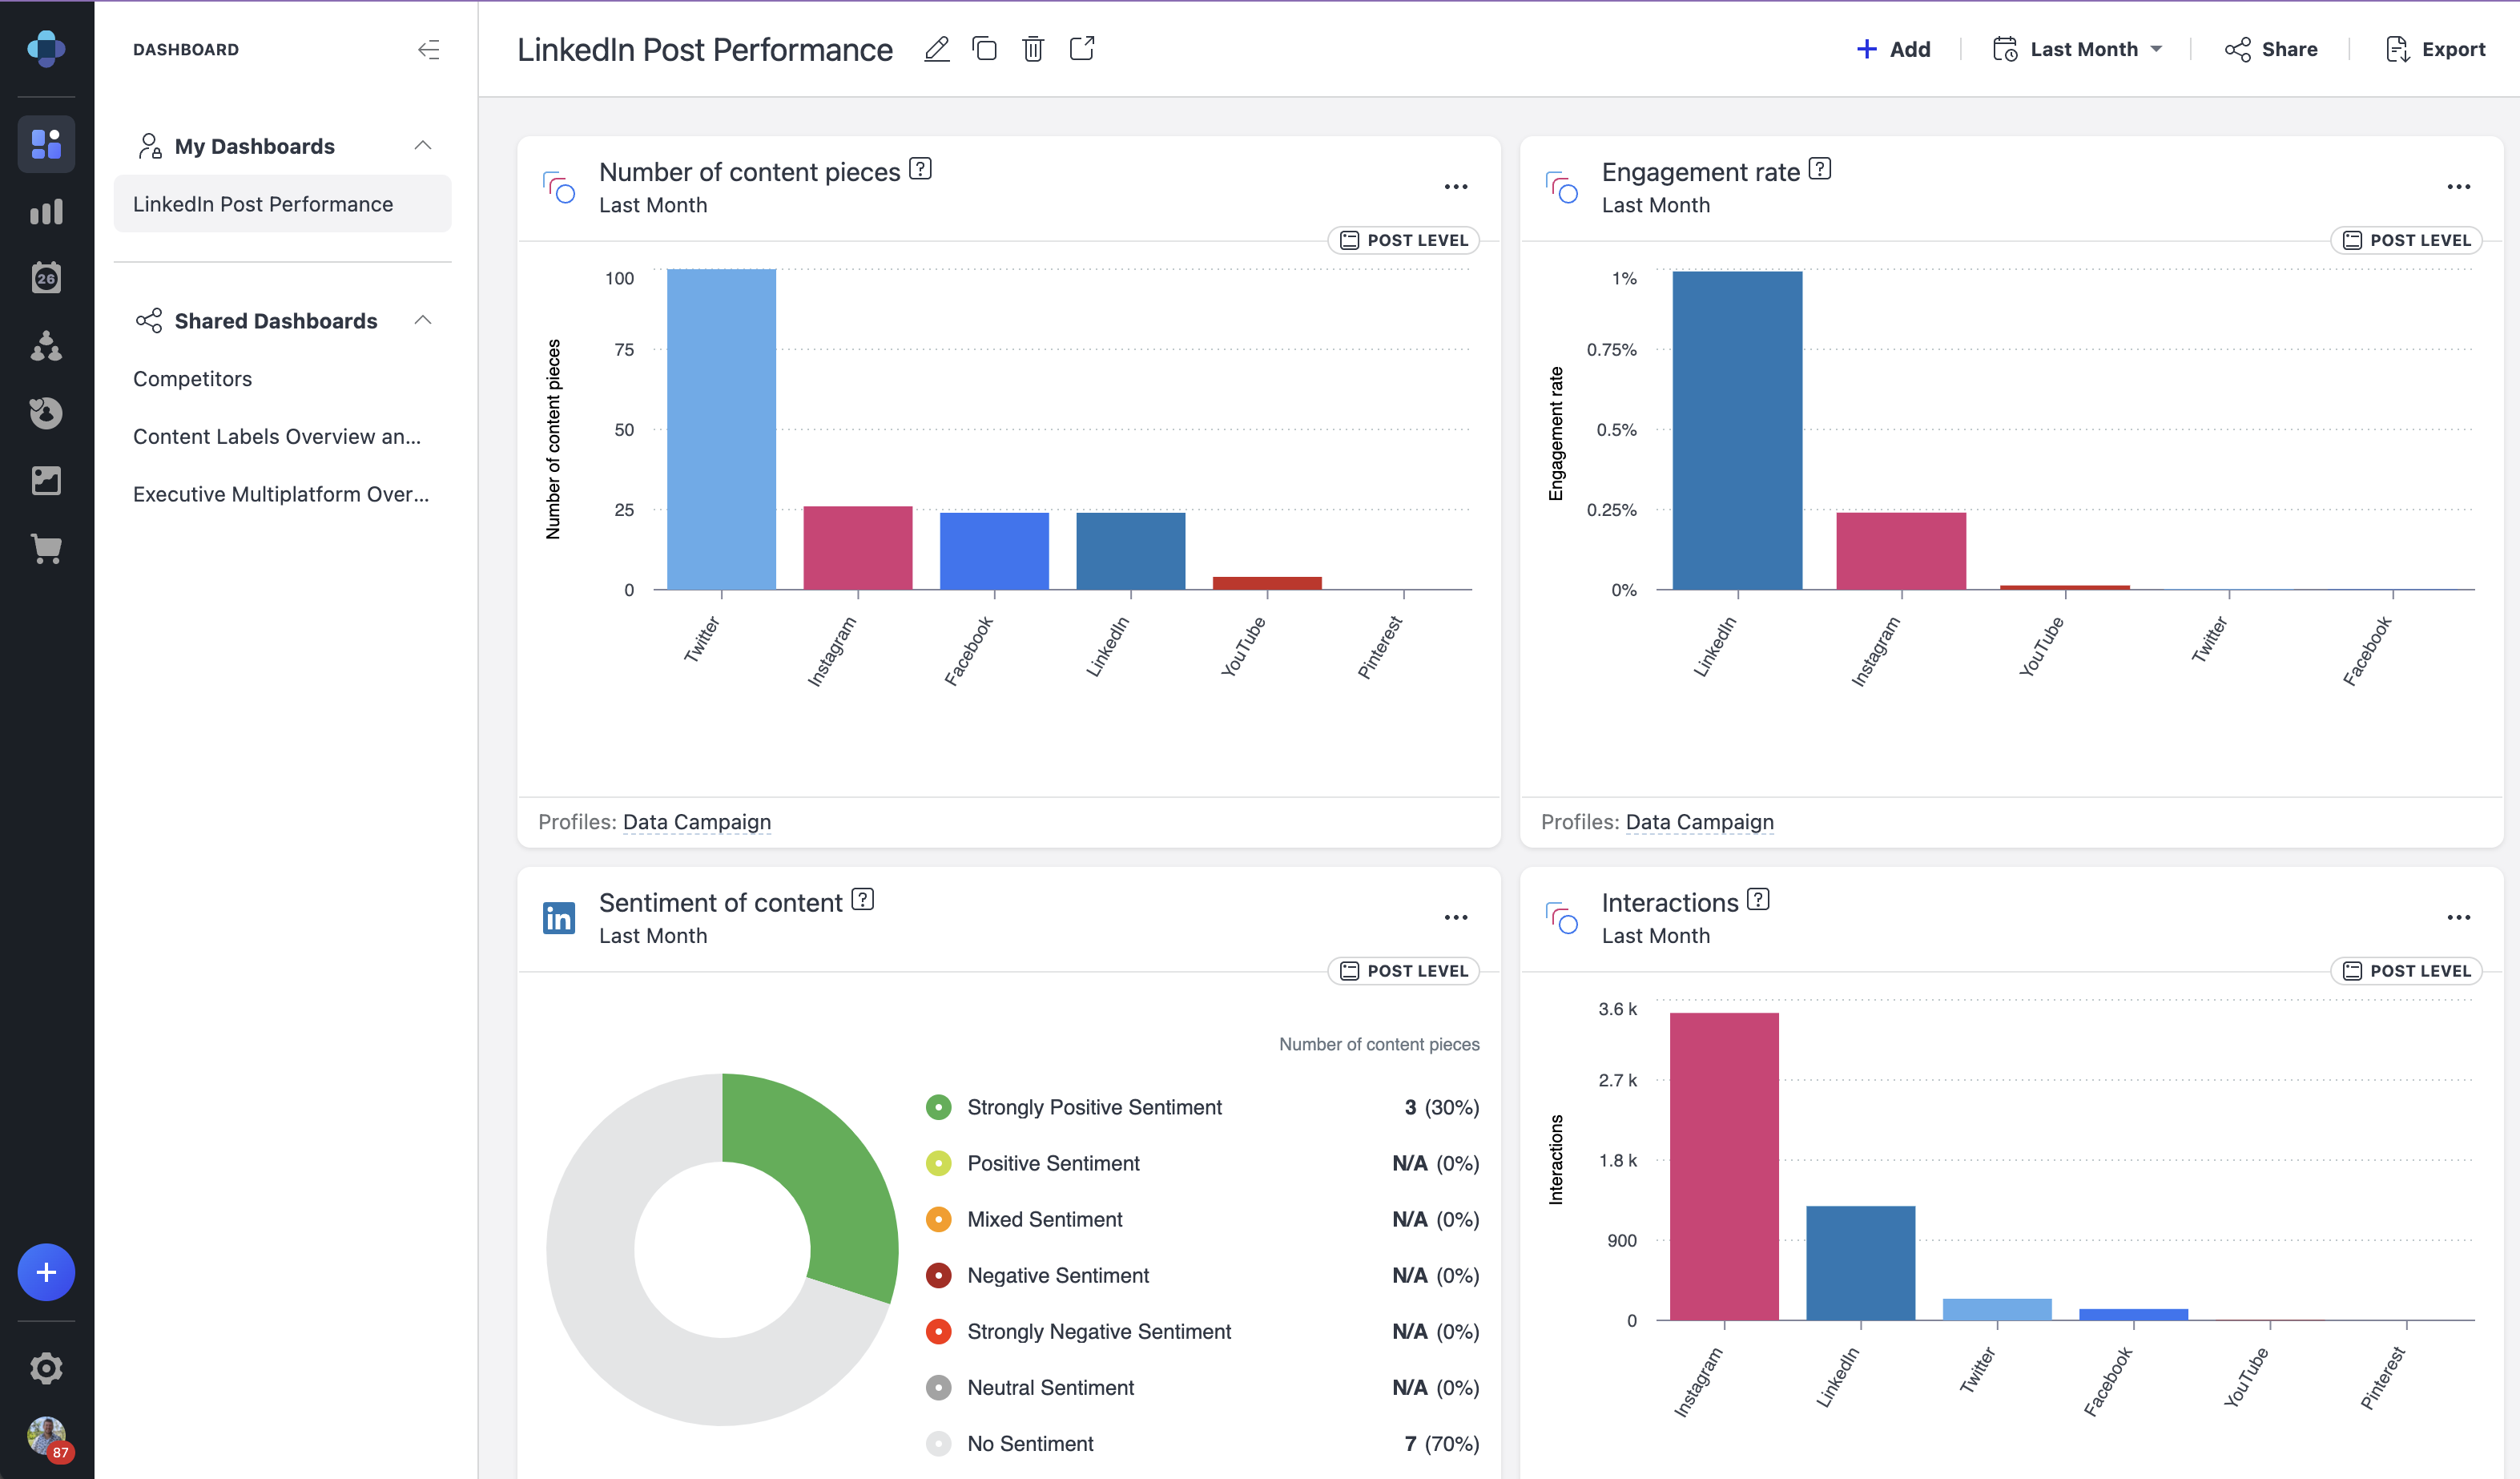
\includegraphics[width=1\textwidth]{pictures/emplifi-dashboard-example.png}
	\caption{Ukázka dashboardu v produktu firmy Emplifi \cite{emplifidashboardIMAGE}}
	\label{fig:emplifiDashUkazka}
\end{figure}

Na obrázku \ref{fig:emplifiDashUkazka} vidíme příklad dashboardu - skládá se z několika grafů, obvykle nazývané jako widgety \cite{emplifiDashboard}, jejichž obsah lze modifikovat pomocí přepínačů v liště. Obsah může být modifikován v časovém období (posledních 30 dní, poslední rok, konkrétní časový rozsah, ...), ale lze jej modifikovat také na základě metrik jako je např. sociální síť (Facebook, Instragram, LinkedIn), druh interakcí (komentáře, liky, sdílení) apod.\footnote{Widgety nemusí být obecně pouze vizualizace, může se jednat také o ovládací prvky (např. výběrové seznamy, check boxy, textfieldy apod.). Tato možnost se využívá zejména ve vývojářských dashboardech pro rychlejší tvorbu vizualizací. V samotném produktu firmy se ale používá kvůli uživatelské přívětivosti pouze pro vizualizace \cite{emplifiDashboard}. 
}

Embedded analytics se nechová a nevypadá jako samostatná aplikace, ale je integrován do jiného softwaru nebo webového portálu. Koncoví uživatelé často ani nepoznají, že se jedná
integrovanou analytiku a vnímají software s touto integrovanou analytikou jako jeden nástroj \cite{goodDataEmbedded}. To umožňuje softwarovým společnostem získat a plně
integrovat analytickou platformu s jejich vlastním SaaS produktem bez nutnosti velkých investic do vývoje vlastního řešení. 

SaaS (Software as a Service) je licenční model, v němž přístup je poskytován na základě předplatného, přičemž software je umístěn na externích serverech, nikoli na firemních serverech \cite{saasDefinition}.
K těmto službám se běžně přistupuje prostřednictvím webového prohlížeče s přihlašovacím jménem a heslem. Výhodou je, že místo toho, aby mělo každé zařízení ve firmě nainstalované
tento program, stačí se do programu přihlásit přes internet. Pro firmu to znamená úsporu financí, jelikož nemusí investovat do nového hardwaru, na němž by dané programy běžely. 
Nevýhodou SaaS je bezpečnost dat a rychlost jejich doručování. Protože jsou data umístěna na externích serverech, je třeba zajistit rychlé a spolehlivé internetové připojení a vyloučit
přístup neoprávněných uživatelů.

Existuje hned několik způsobů, jak data embedovat. Mezi nejpopulárnější a nejrozšířenější způsoby patří HTML iframe, webová komponenta či React SDK s voláním API \cite{goodDataEmbedded}. 

\subsection{Iframe}
Nejjednodušší a nejrychlejší metodou embedování je využití použití iframu \cite{goodDataEmbedded}. Iframe (inline frame) je HTML prvek, který umožňuje načíst HTML stránku uvnitř dokumentu \cite{iFrameAdv}. Používá se pro vložení určitého obsahu z jednoho zdroje do druhého. To se poté jeví jako nové okno v dané stránce, jedná se ovšem o embedovaný iframe. Tuto možnost embedování využívají např. Google Mapy nebo YouTube \cite{iFrameAdv}. Velkou výhodou je, že není třeba instalovat pro běh žádné dependence.

\subsection{Webová komponenta}
Pokročilejší technikou pro embedování je použití webové komponenty. Výhoda opět spočívá v tom, že není třeba instalovat závislosti pro běh. Embedování probíhá pomocí knihovny, která se naimportuje přes HTML tag \texttt{<script>}. Poté je možno embedovat vizualizace pouze prostřednictvím naimplementovaných webových komponent \cite{webComp}.

\subsection{React SDK + API}
Poslední zmiňovanou možností je embedování prostřednictvím React SDK s voláním API. 

SDK (Software development kit) je označení sady nástrojů pro tvorbu softwaru \cite{SDKvsAPI}, které umožňuje vývojářům vytvářet rychleji a standartizovaně nové aplikace. API 
(Application Programming Interface) je rozhraní usnadňující komunikaci mezi dvěmi platformami. Uživatel specifikuje požadavek na data, rozhraní API provede volání na webový server, který
následně tento požadavek zpracuje a odešle odpověď na specifikované volání (může se jednat např. o data ve formátu JSON). Díky tomu se krátí vývojový cyklus (automatizace), efektivně 
se poskytují nové služby uživatelům a může zlepšit reputaci důvěryhodnost značky.

K embedování je potřeba následovat instrukce (např. nainstalování dependencí, zprovoznění backendu apod.) a zajistit, že všechny kroky v nich obsažené budou splněny \cite{reactSDKComp}. Jedná se tedy o programátorsky náročnější metodu, ovšem výhoda spočívá ve větší flexibilitě vývojářů, kteří mohou vizualizace snadno modifikovat \cite{goodDataEmbedded}.

%
% Podkapitola zabezpečení
%
\section{Zabezpečení}
Zabezpečení API je důležitou součástí v moderním inženýrství zajišťující bezpečnou a důvěryhodnou komunikaci mezi různými aplikacemi. S rostoucím významem API pro výměnu dat mezi
systémy je nezbytné věnovat zvláštní pozornost implementaci efektivních bezpečnostních opatření. API authentication (autentizace) je řešením pro ověřování uživatelů - to umožňuje
vlastníkovi daného API ochranu před neoprávněným přístupem ze strany uživatelů, kteří nemohou ověřit svou totožnost \cite{whatIsAPI}.

Řešení autentizace jsou obvykle nastavena tak, aby zablokovala přístup do API, pokud se při volání zjistí něco nesprávného či nevalidního s uživatelem. S tím se pojí druhá bezpečnostní
složka, kterou je autorizace (authorization). Zatímco autentizace ověřuje identitu uživatele, autorizace se zabývá tím, jaké akce má daný uživatel povoleny \cite{mostUsedAuthentication}. 
Mezi nejpoužívanější metody patří HTTP authentication, API keys a OAuth 2.0. 

\subsection{HTTP autentizace}
HTTP autentizace omezuje přístup k serveru pomocí předdefinovaných schémat. 

Jedním z používaných schémat je Basic HTTP \cite{mozillaHTTPAuth}. Uživatel, který chce ověřit svou identitu, tak může učinit vložením hlavičky 
Authorization s bezpečnostními údaji - nejčasteji tím bývá uživatelské jméno a heslo. 
Samotné ověřování pomocí HTTP Basic se ovšem nedoporučuje. Přenášené údaje jsou sice zakódované, ale nejsou zašifrované \cite{mozillaHTTPAuth}. Proto je třeba v případě použití zajistit šifrované spojení (HTTPS/TLS). Atribut hlavičky se zakódovaným uživatelským jménem a heslem může vypadat např. jako na ukázce \ref{basicHeader}.

\begin{lstlisting}[language=json, caption={Autorizační atribut - Basic schéma}, label=basicHeader]
	Authorization: Basic drgnpdrgud653==,
\end{lstlisting}

Bearer schéma obsahuje tzv. bearer tokeny. Bearer token specifikuje, k jakým zdrojům může uživatel v API přistupovat \cite{mostUsedAuthentication}. Token je obvykle řetězec vygenerovaný serverem v reakci na požadavek na přihlášení. Opět je nutné zajistit zabezpečené spojení jako v případě Basic schématu. Atribut hlavičky s tokenem může vypadat např. jako na ukázce \ref{bearerHeader}

\begin{lstlisting}[language=json, caption={Autorizační atribut - Bearer schéma}, label=bearerHeader]
	Authorization: Bearer se5Edg345dsBNN-7df,
\end{lstlisting}


\subsection{API key}
API klíč (key) je jedinečný alfanumerický řetězec, který slouží k jednoznačné identifikaci klientů/aplikací \cite{amazonAPIKey}, jenž API využívají. Narozdíl od tokenů
nejsou časově omezené - to může znamenat bezpečnostní problém v případě, že při zadávání požadavku API by přenášený klíč mohl být zachycen \cite{mostUsedAuthentication} a s ním i celá síť, pokud by obsahovala jeden nezabezpečený bod. Proto je i v tomto případě nutné zajistit šifrované spojení \cite{keepingApiKeysSafe}.
Pokud API bude sloužit pouze ke čtení, je zabezpečení API klíčem tou nejlepší volbou - uživatelé budou moci data stahovat, ale nikterak modifikovat či mazat \cite{mostUsedAuthentication}. 

\subsection{OAuth}
OAuth (Open Authorization) protokol byl vyvinut jako řešení pro udělování přístupu na předem definovanou dobu bez sdílené uživatelských jmen a hesel \cite{understandingOAuth2}. OAuth 2.0
je nejlepší volbou pro identifikaci osobních uživatelských účtů a udělování patřičných oprávnění \cite{mostUsedAuthentication}. Proces autentizace je vidět na obrázku \ref{fig:oauth2Diagram}.


\begin{figure}
	\centering
	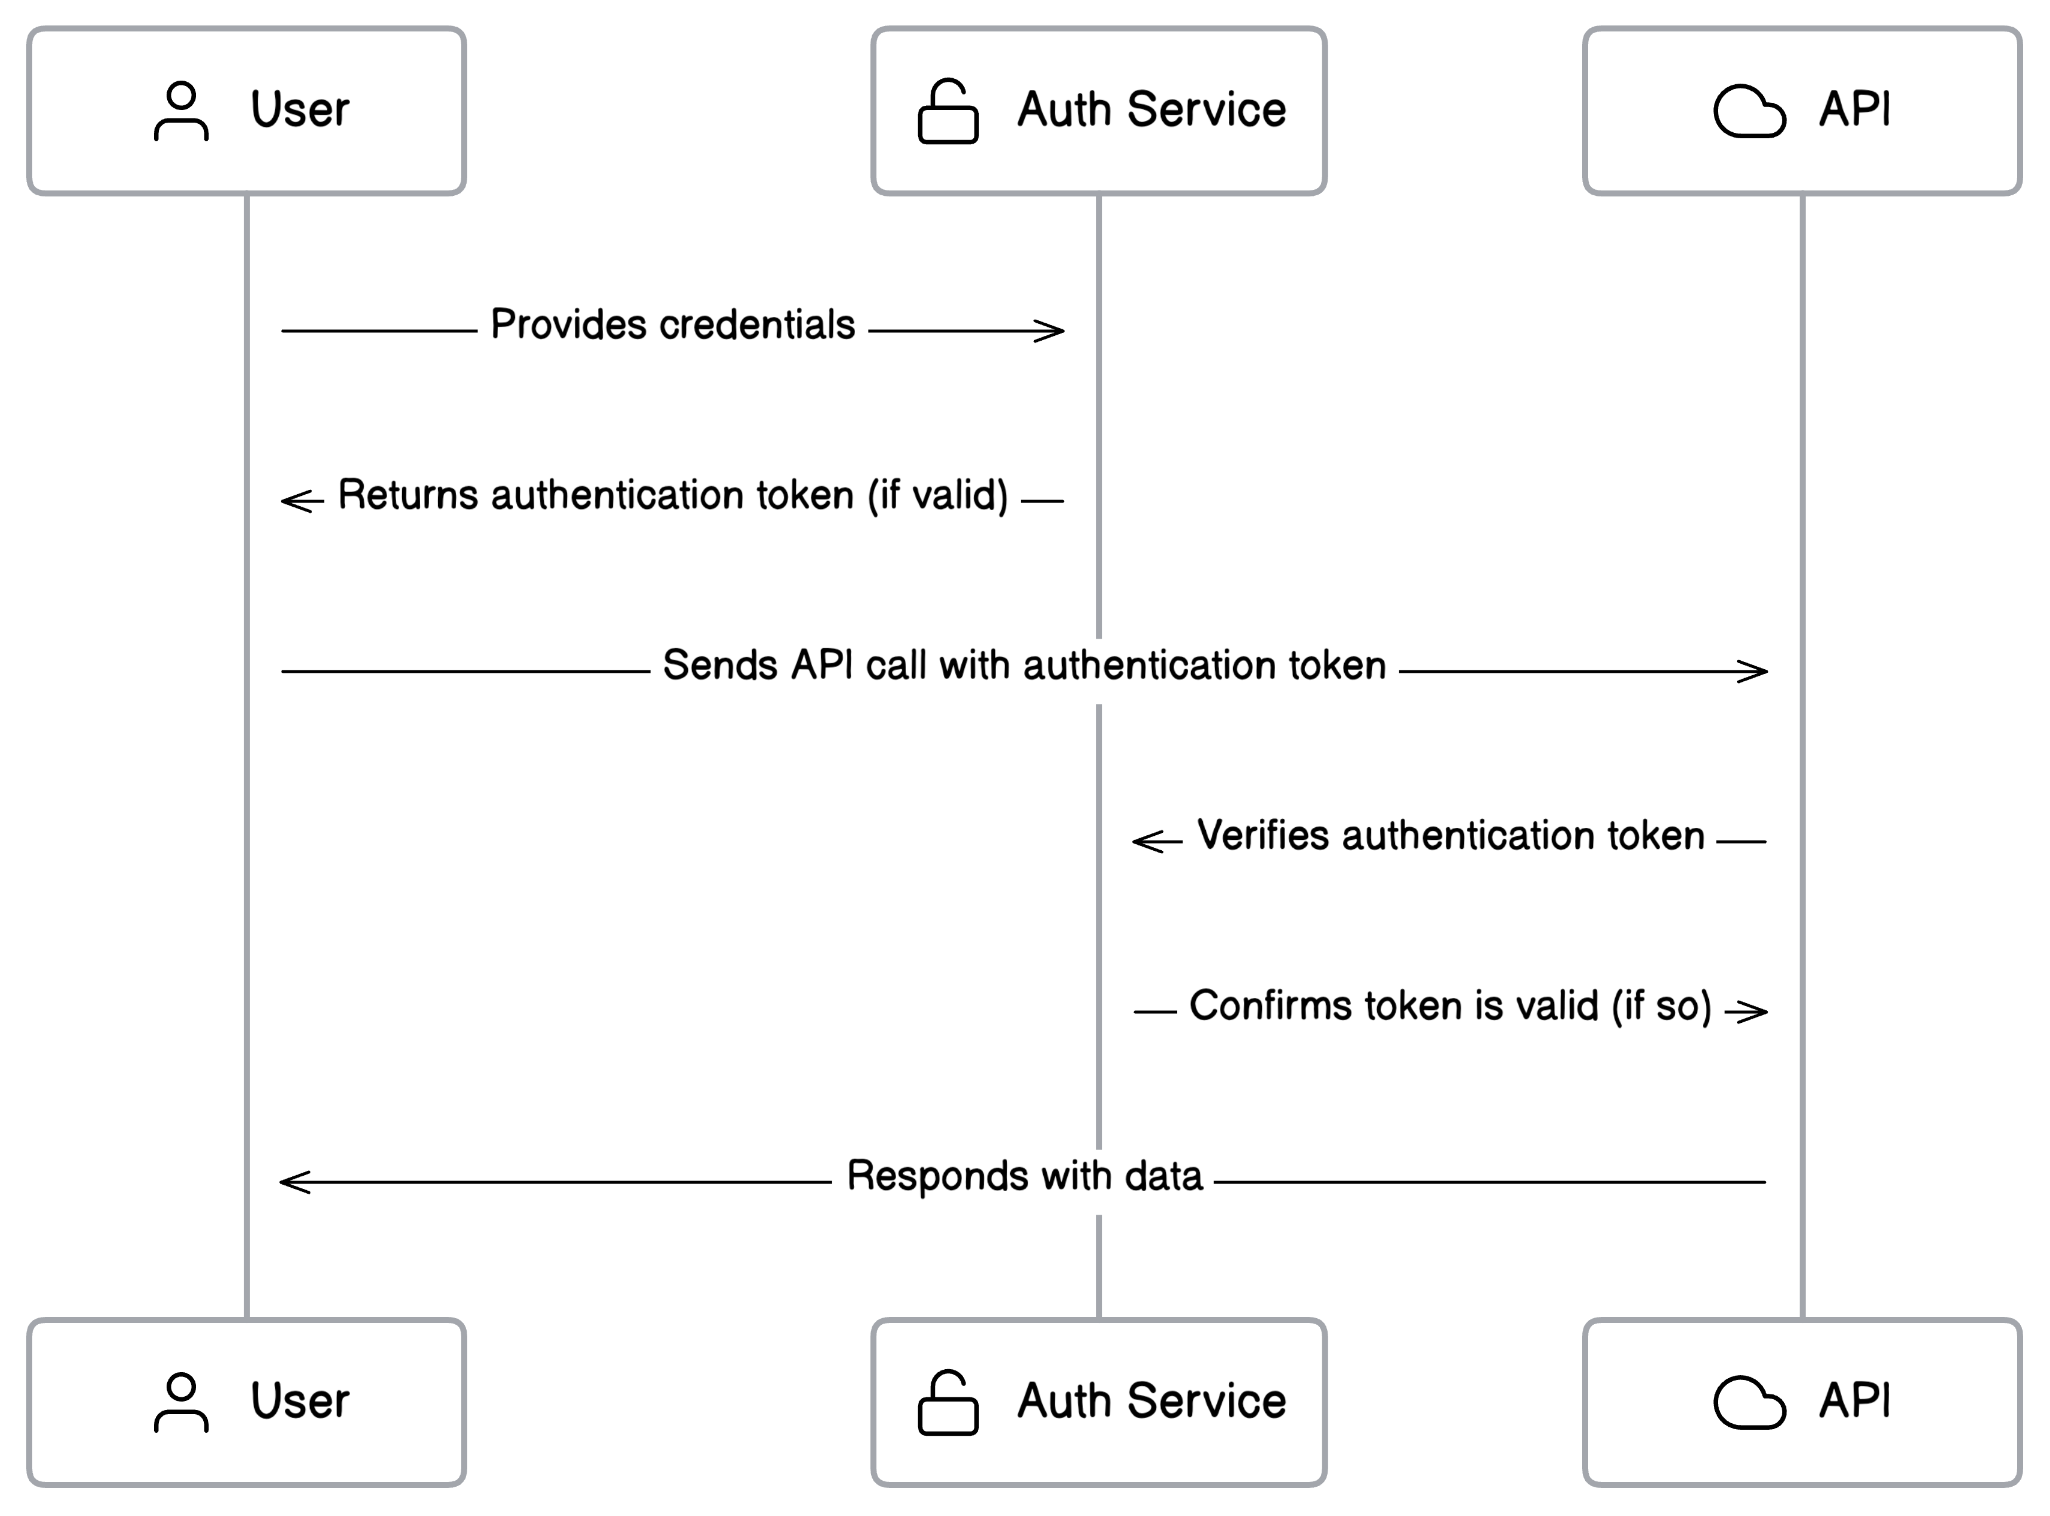
\includegraphics[width=1\textwidth]{pictures/oauth2-diagram.png}
	\caption{Autentizační diagram protokolu OAuth 2.0 \cite{oAuthImage}}
	\label{fig:oauth2Diagram}
\end{figure}


Nejprve se uživatel přihlásí do systému - nejčastěji formou uživatelského jména a hesla, nebo klientského id a secretu. Tím se pošle HTTP požadavek na endpoint. Autorizace uživateli následně
vrátí token. Pokud má uživatel již platný token, může přistupovat k datům. Naopak pokud mu token již expiroval nebo není platný, volání do API mu vrátí chybové hlášení. 

Součástí autorizační odpovědi bývá i několik dalších údajů. Odpověď může vypadat např. jako na \ref{tokenResponse}. 

\begin{lstlisting}[language=json, caption={Ukázková odpověď autorizačního serveru}, label=tokenResponse]
{
	"access_token": "G7k4Q2s1bD5z9x",
	"token_type": "Bearer",
	"expires_in": 3600,
	"refresh_token": "5aB3c9Cx8P5y2z",
	"scope": "create"
}
\end{lstlisting}
	  
Odpověď bývá ve formátu JSON (JavaScript Object Notation) a obsahuje informace o daném přístupovém tokenu (access\_token). Kromě přístupového tokenu obvykle obsahuje i refresh\_token. Ten umožňuje uživateli 
používat stále jeden token bez nutnosti generování nového \cite{oauthResponseExample}. Dále může obsahovat specifikující práva uživatele (scope), platnost tokenu (expires\_in) či typ tokenu (token\_type), jež některé z nich byly zmíněny v předchozí kapitole.
Přesný formát odpovědi je ale specifikován samotným API - tudíž každé API může mít jiné délky přístupových a obnovovacích tokenů, časové platnosti tokenů či i samotné atributy v odpovědi a jejich názvy.
%
% Podkapitola existující řešení
%
\section{Existující řešení}
Embedded analytics problematikou se zabývá mnoho firem a každá z nich disponuje jinými způsoby řešení. Zde budou zmíněny firmy, které se objevují často na vrchních příčkách
internetových recenzí či firmy, které byly pro inspiraci doporučeny externím zadavatelem. Pro aktuálnost jsou brány informace ze zdrojů z roků 2022/2023.
\subsection{GoodData}
Firma GoodData byla zmíněna zadavatelem jako jedna z nejvýraznějších na trhu. Dodává embedded analytics systémy firmám jako je VISA, Zalando či Bentley \cite{goodDataEmbeddingPlatform}. 
Embedování provádí třemi zmíněnými způsoby - HTML iframem, webovou komponentou či React SDK. Zákazníkům nabízí přizpůsobení dashboardů tak, aby odpovídaly zákazníkovo značce. GoodData získaly
v roce 2023 hned několik ocenění firmou TrustRadius, důvěryhodnou platformou v oblasti B2B (bussines to bussines) \cite{trustRadiusDiscusionGoodData}. Firma GoodData obdržela ocenění Best Value for Price,
Best Relationship či Top Rated 2023. Zákazníci firmy GoodData si v recenzích chválí hlavně snadné používání, zákaznickou podporu, širokou škálu podporovaných databází či uživatelsky přívětivé
rozhraní \cite{trustRadiusDiscusionGoodData}. Naopak se zmiňují, že dokumentace může být nedostačující či některé endpointy v API mají neintuitivní parametry. I tak ale 92\% recenzentů uvádí,
že by si produkt zakoupili znovu.

\subsection{Microsoft Power BI}
Mezi často zmiňovaným produktem je Microsoft Power BI, který je ve svém oboru nejlepší v oblasti bezpečnosti a zabezpečení \cite{bestEmbTools2023},
jelikož Microsoft zaměstnává více než 3500 bezpečnostních expertů. V produktu nabízí také tzv. playground, který
umožňuje uživatelům testovat funkce a vlastnosti daných dashboardů před úplným nasazením. Je také podporvána integrace s cloudovou službou Microsoft Azure. Na webu TrustRadius je k 
Microsoft Power BI podstatně méně recenzí než k produktu GoodData (5x méně). Uživatelé zmiňují dlouhou dobu při zpracování většího objemu dat či vysokou provozní cenu \cite{trustRadiusDiscusionAzure}.

\subsection{Powered by Looker}
V oblasti modelování data vyniká platforma Powered by Looker \cite{bestEmbTools2023}. Jedná se o produkt služby Google Cloud, který poskytuje způsob, jak sledovat změny a prohlížet jejich
historii v databázi. Disponuje modelovacím jazykem LookML založeným na SQL, který slouží k vytváření sémantických datových modelů. Pomocí něj lze popisovat jednotlivé dimenze, agregáty,
výpočty či datové vztahy v databázi \cite{googleLookMLDoc}. Z toho vyplývá, že datové modely jsou rozšiřitelné, opakovatelně použitelné a konzistentní a tudíž efektivní. V roce 2022 byl tento produkt
oceněn Top Rated a Most Loved společností TrustRadius \cite{trustRadiusDiscusionLooker}. Uživatelé zmiňují, že produkt může být pomalejší a že nástroje na přizpůsobení dashboardů by mohly být
vylepšeny a rozšířeny.


\subsection{Tableau}
Tableau vyniká ve vytváření estetických a interaktivních vizualizací \cite{tableauBlog}. Dále nabízí zákazníkům publikaci vizualizací prostřednictvím produktu Tableau Online. Cena produktu začíná na \$70 měsíčně za jednoho uživatele \cite{trustRadiusTableAU}. 
Zákazníci produkt hodnotí velmi kladně - 100\% z nich uvádí, že implementace proběhla jak očekávali, 98\% jsou s výsledkem spokojeni a 91\% by si tento produkt zakoupilo zase \cite{trustRadiusTableAU}. Silné stránky 
tohoto produktu spočívají v automatickém generování kódu pro embedování a jednoduché vkládání dashboardů do webových stránek \cite{tableauBlog}. Kritika naopak zaznívá na zákaznickou podporu či pomalé načítání při velkém množství dat \cite{trustRadiusTableAU}.

% _____________________________________________________________________________
%
%
%        CHAPTER Návrh knihovny
%
% _____________________________________________________________________________
%
\chapter{Návrh knihovny a uživatelského rozhraní}

V této kapitole bude popsán detailní návrh knihovny, uživatelského rozhraní a technologie, jež budou použité k realizaci. 

\section{Technologie}

\subsection{JavaScript a React}
Pro vývoj knihovny bude využit JavaScript s knihovnou React. Důvodem zvolení těchto technologií je požadavek ze strany zadavatele. React a JavaScript jsou dnes
široce používané technologie ve vývoji webových aplikací. 

React je snadný na naučení, obsahuje málo konceptů, které je třeba se naučit \cite{whyUsingReact}. Jeho instalace je snadná -
stačí pouze v kódu nainstalovat a naimportovat jeho knihovnu. Využívá speciální JSX syntaxe, která sice vypadá jako HTML, ale ve skutečnosti je tato syntaxe převáděna na HTML. Jelikož je React hojně využíván
v aplikaci Facebook či na Instagramu, dostává se mu velké podpory právě i z tohoto odvětví - čtyři největší přispěvatelé knihovny React jsou zaměstnanci Facebooku \cite{whyUsingReact}. Kromě 
Facebooku využívají React značky jako jsou např. Netflix, airbnb, BBC News či PayPal \cite{whyUsingReact2}. Díky virtualizaci a uchováváním DOM poskytuje React
velmi rychlé vykreslování, přičemž všechny změny se snadno promítají do virtuálního DOM. 

DOM (Document Object Model) je strukturovaná reprezentace jazyka HTML, které reprezentuje celé uživatelské rozhraní jako stromovou datovou strukturu \cite{whatIsDOM}. Každý prvek uživatelského
rozhraní tvoří v DOM stromu právě jeden uzel. Dojde-li ke změně uživatelského rozhraní, DOM se aktualizuje 	a při každé změně se vykresluje znovu, což výrazně ovlivňuje výkon aplikace. 
Toto lze vyřešit použitím virtuálního DOM. Při přidávání nových věcí do aplikace se vytvoří virtuální DOM, která je reprezentován jako strom. Novější virtuální DOM se porovnává se starším, aby
zaznamenal změny. Poté zjistí, jak je možné tyto změny provést pomocí skutečného DOM a aktualizované prvky se následně vykreslí.

React využívá tzv. komponent, které slouží k vizualizaci aplikace \cite{introToReact}. Existují dva druhy těchto komponent - funkcionální a třídní \cite{functionalVsClass}. Knihovna bude používat funkcionální, jelikož
se jedná o novější verzi komponent.

Na popularitě Reactu přidává také použití knihovny Redux, která umožňuje uchování dat jako jeden objekt (stav). Použití Reduxu je vhodné zejména u velkých aplikací - čím větší je aplikace, tím
náročnější je správa stavu aplikace \cite{introToRedux}. K reduxovému stavu objektu se dá pak jednoduše přistupovat, což značně usnadňuje práci s daty.
Je-li tento stav změněn, aplikace se překreslí a zobrazení se stále synchronizuje se souvisejícími daty \cite{whyUsingReact2}. 

React se kvůli těmto vlastnostem doporučuje využívat u:
\begin{enumerate}
\item Obsáhlých uživatelských rozhraní
\item Rozsáhlých aplikací
\item Aplikací náročné na výkon
\item Multi-platformních aplikací
\end{enumerate}

Na frontend komponent knihovny a rozhraní pro obnovu tokenů bude použita knihovna MUI, která nabízí širokou škálu předdefinovaných komponent a stylů \cite{muiDocs}. 	

\subsection{Emplifi API}	
Data potřebná k embedování grafů budou získávána prostřednictvím Emplifi Public API. 
Toto rozhraní poskytuje klientům snadný a oblíbený způsob, jak získat přístup k potřebným datům. 
Emplifi API se nachází na veřejné webové adrese a žádat o data může každý, kdo má přístupový token.
Struktura dotazů a ukázkové dotazy jsou dostupné na veřejné dokumentaci \cite{emplifiDocs}.

\subsubsection{Vytvoření tokenu}

Vytvoření tokenu je umožněno pouze osobám, jež mají u firmy Emplifi vytvořený účet v produktu Suite. Na diagramu \ref{fig:emplifAPIDiagram} je schéma, které udává průběh akcí během žádání o 
přístupový token a zaslání prvního requestu s žádostí o data.
\begin{figure}
	\centering
	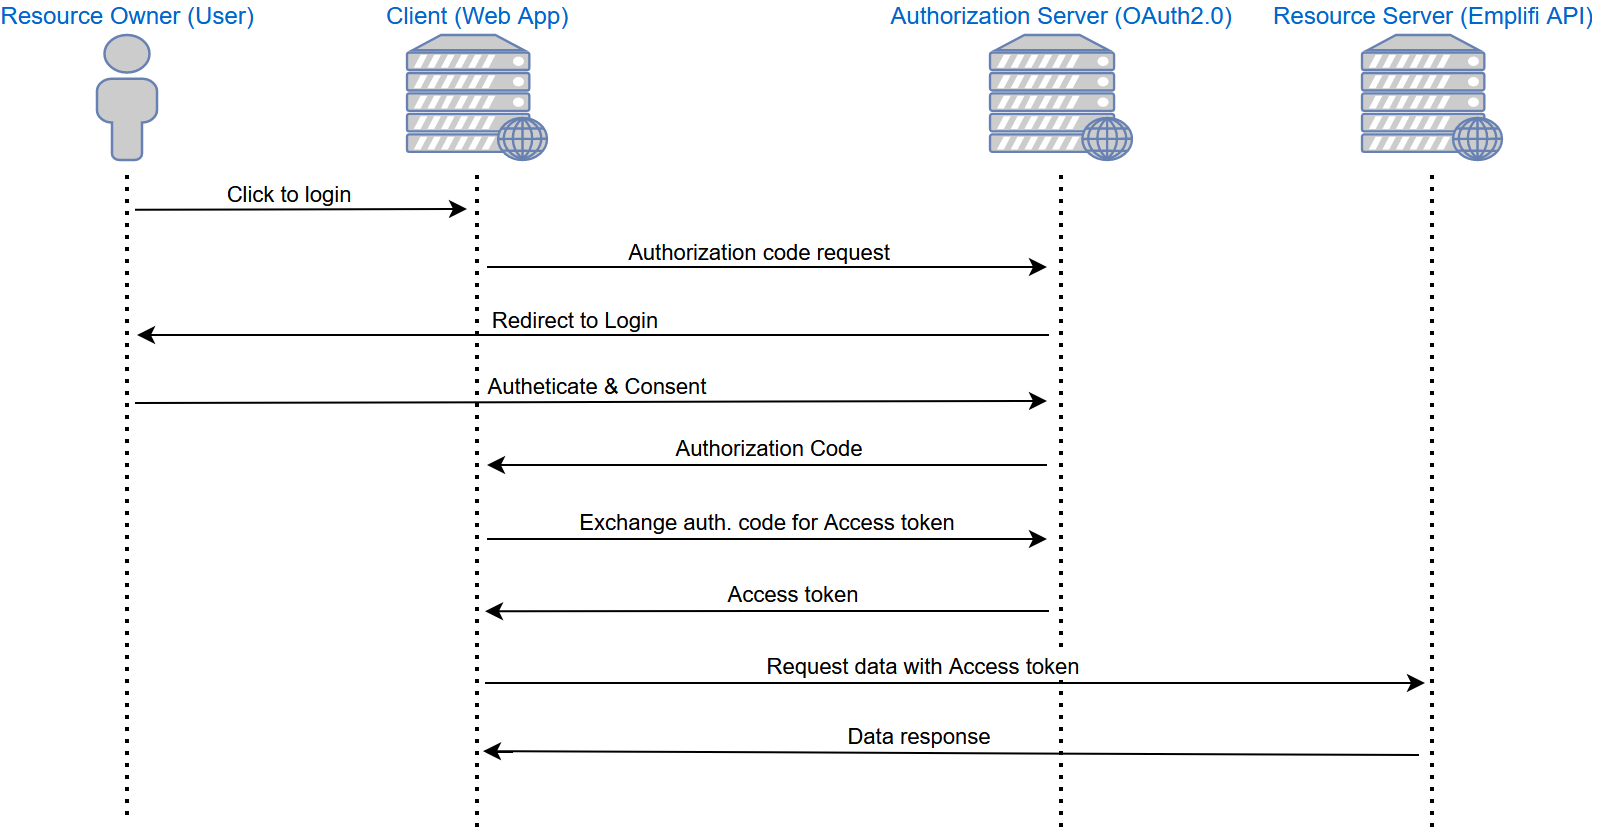
\includegraphics[width=1\textwidth]{pictures/emplifiAPI.png}
	\caption{Diagram vytvoření Emplifi API tokenu \cite{emplifiDocs}}
	\label{fig:emplifAPIDiagram}
\end{figure}

Pro vytvoření tokenu je třeba uživatele přesměrovat na webovou URL \url{https://api.emplifi.io/oauth2/0/auth}, kde bude požádán o udělení souhlasu z jeho Emplifi Suite účtu.
Do URL, na kterou uživatele přesměrujeme, bude třeba vložit několik parametrů potřebných k autentizaci a k následnému vrácení tokenu. 

\begin{center}
	\begin{longtable}{p{.2\textwidth}p{.65\textwidth}}
	\caption{Seznam všech parametrů vkládaných do URL adresy při tvorbě tokenu \cite{emplifiDocs}}
	\label{tab:allParametersAPI}\\
	\toprule[1.5pt]
	\endhead
	\midrule
	\multicolumn{2}{r}{\textit{(tabulka pokračuje na další stránce)}}\\
	\endfoot
	\bottomrule[1.5pt]
	\endlastfoot
	%
	\verb"client_id" &  Jedinečný klientský identifikátor pro aplikaci.\\
	\midrule
	\verb"redirect_uri" & Návratová adresa. Na tuto adresu bude při úspěšné autorizaci přesměrován přístupový token. Zároveň tato adresa musí být povolena vývojáři v interní databázi.\\
	\midrule
	\verb"response_type" & Typ - Emplifi momentálně podporuje pouze hodnotu "code".\\
	\midrule
	\verb"scope" & Specifikuje prostředky oddělené mezerou, ke kterým aplikace může přistupovat klientským účtem. Ty při udělování souhlasu budou předloženy ke schválení. \\
	\midrule
	\verb"state" & Hodnota sloužící k validaci přijaté odpovědi. Při zaslání requestu je vložena hodnota do parametru, autorizační server jí při zpracování dotazu odešle zpět s daty. Uživatelská aplikace by následně měla porovnávat, zda tato zaslaná hodnota je shodná s původní - to slouží k zabránění útoků Cross-site Request Forgery.\\
	\midrule
	\verb"prompt" & Musí být nastavena na hodnotu "consent", pokud má být refresh token vrácen společně s přístupovým.\\
	\end{longtable}
\end{center}


Pokud veškeré parametry budou správně nastaveny a uživatel udělí souhlas s používáním Suite účtu, na URL "redirect\_uri" se vrátí zpráva s autorizačním kódem. Tento kód
slouží k výměně za přístupový token. O ten je možno si zažádat POST requestem na adresu \url{https://api.emplifi.io/oauth2/0/token}. Struktura requestu je popsána v tabulkách \ref{tab:exampleRequestHeader} a \ref{tab:exampleRequestBody}.

\begin{center}
	\begin{longtable}{p{.2\textwidth}p{.65\textwidth}}
	\caption{Hlavička requestu na token \cite{emplifiDocs}.}
	\label{tab:exampleRequestHeader}\\
	\toprule[1.5pt]
	\endhead
	\midrule
	\multicolumn{2}{r}{\textit{(tabulka pokračuje na další stránce)}}\\
	\endfoot
	\bottomrule[1.5pt]
	\endlastfoot
	%
	\verb"Authorization" & Řetězec "Basic" s klientským identifikátorem a zakódovaným klientským secretem oddělený dvojtečkou v Base64. Výsledná hodnota vypadá např. takto: "Basic Y2xpZW50X2lkOmNsaWVudF9zZWNyZXQ=."\\
	\midrule
	\verb"Content-Type" & Hodnota "application/x-www-form-urlencoded" \\
	\end{longtable}
\end{center}

\begin{center}
	\begin{longtable}{p{.2\textwidth}p{.65\textwidth}}
	\caption{Tělo requestu na token \cite{emplifiDocs}.}
	\label{tab:exampleRequestBody}\\
	\toprule[1.5pt]
	\endhead
	\midrule
	\multicolumn{2}{r}{\textit{(tabulka pokračuje na další stránce)}}\\
	\endfoot
	\bottomrule[1.5pt]
	\endlastfoot
	%
	\verb"code" & Řetězec sloužící k následné validaci při zpětném volání. \\
	\midrule
	\verb"grant_type" & Hodnota "authorization\_code" \\
	\midrule
	\verb"redirect_uri" & URL adresa, kam bude přesměrován token. Musí být stejná jako v tabulce \ref{tab:allParametersAPI} \\
	\end{longtable}
\end{center}

Následně obdržíme token ve formátu jako na \ref{tokenResponse}. Přesné návratové hodnoty jsou popsány v tabulce \ref{tab:exampleRequestResponse}.

\begin{center}
	\begin{longtable}{p{.2\textwidth}p{.65\textwidth}}
	\caption{Tělo odpovědi se zaslaným tokenem \cite{emplifiDocs}.}
	\label{tab:exampleRequestResponse}\\
	\toprule[1.5pt]
	\endhead
	\midrule
	\multicolumn{2}{r}{\textit{(tabulka pokračuje na další stránce)}}\\
	\endfoot
	\bottomrule[1.5pt]
	\endlastfoot
	%
	\verb"access_token" & Přístupový token k Emplifi Public API. \\
	\midrule
	\verb"token_type" & Jediný podporovaný typem je "bearer". \\
	\midrule
	\verb"expires_in" & Platnost tokenu ve vteřinách. \\
	\midrule
	\verb"refresh_token" & Token pro obnovení přístupového tokenu. Zaslán pouze v případě, pokud \verb"scope" obsahuje řetězec "offline\_access".\\
	\midrule
	\verb"scope" & Prostředky, které byly uživatelem uděleny. Odděleny mezerou. \\
	\end{longtable}
\end{center}



Užívání tokenů má ovšem nastavené limity - 500 requestů za hodinu pro uživatele, 1000 requestů za hodinu pro účet \cite{emplifiDocs}. Pokud bude tato hranice přesažena,
API vrátí odpověď s informací, že uživatel či účet překročili maximální limit dotazů.

\subsubsection{Endpointy}

Má-li uživatel platný token, může začít se zasíláním dotazů. Emplifi API disponuje množstvím endpointů, přičemž endpointy využívané k embedování jsou zmíněné v tabulce \ref{tab:embeddingEndpoints}. 

\begin{center}
	\begin{longtable}{p{.25\textwidth}p{.6\textwidth}}
	\caption{Endpointy používané k embedování.}
	\label{tab:embeddingEndpoints}\\
	\toprule[1.5pt]
	\endhead
	\midrule
	\multicolumn{2}{r}{\textit{(tabulka pokračuje na další stránce)}}\\
	\endfoot
	\bottomrule[1.5pt]
	\endlastfoot
	%
	\verb"/3/omni/metrics" & Získávání dat pro vizualizace. Data jsou ve formátu omni. \\
	\midrule
	\verb"/3/omni-studio" &  Získávání widget konfigurací, fieldů a vytváření Omni API tokenů\\
	\midrule
	\verb"/oauth2/0" &  Vytváření Public API tokenů. \\
	\end{longtable}
\end{center}

Endpoint omni-studio bylo nutné vytvořit zadavatelem, jelikož Omni API endpointy bylo možné volat pouze při použití firemní VPN. Nyní lze tyto endpointy provolávat prostřednictvím Public API. Původní
strukturu Omni API requestu lze vložit do těla public API requestu, což umožní uživateli embedovat grafy i mimo VPN.

\subsubsection{Knihovny pro fetchování dat}

V současné době existuje mnoho knihoven určené pro fetchování dat. Data bude nejprve nutné načíst na backend běžící aplikace, která je následně vrátí na frontend. Na backendu probíhá fetchování dvojím způsobem - 
využitím zabudovaného fetch API v Node.js a knihovnou axios. Pro načítání dat z backendu na frontend budeme využívat rozhraní JavaScriptu Fetch API a knihovnu TanStack React Query. Její výhodou je cachování
requestů \cite{tanstackQueryDocs} - pokud byl poslán jednou již stejný dotaz na data, načtení dat neproběhne z API, ale z uložené cache. To omezí počet requestů zaslaných na API a zmenší prodlevu vizualizace (data načtou rychleji z cache než z API). 

\subsection{PreJSON a Vision}

Interní knihovny, které budou využiti k upravování widget konfigurací (PreJSON) a následné vizualizaci grafů (Vision).

PreJSON slouží k expandování konfigurací widgetů. Stažené konfigurace widgetů obsahují tzv. preJSON hodnoty, které jsou později dodefinovány uživatelem. Např. je-li stažena konfigurace, která obsahuje
nespecifikovaný parametr, můžeme jej dodefinovat použitím instance PreJSONu \cite{preJSONDocs}. Na zjedodušené ukázce \ref{notExpandedPreJson} je zobrazen PreJSON objekt, který by mohl specifikovat tělo dotazu. 

\begin{lstlisting}[language=json, caption={Neexpandovaný PreJSON objekt}, label=notExpandedPreJson]
{
	customer_id: 12651141417427,
	time: "P30D/now[sD]",
	platform: ${string:platform_name}
}
\end{lstlisting}
		
Atributy \texttt{customer\_id} a \texttt{time} jsou již předdefinové, ale na uživateli zůstává možnost volby parametru \texttt{platform}. Datový typ parametru musí být vždy specifikován.
Zde se očekává string hodnota, která může nabývat (opět pouze pro ukázku) např. hodnot "instragram", "facebook", "snapchat", "linkedin" apod. Uživatel tedy zvolí jednu ze sociálních sítí
a pomocí funkce \texttt{expand()} může tuto hodnotu dodefinovat. Výsledek může vypadat poté jako na ukázce \ref{expandedPreJson}.

\begin{lstlisting}[language=json, caption={Expandovaný PreJSON objekt}, label=expandedPreJson]
{
	customer_id: 12651141417427,
	time: "P30D/now[sD]",
	platform: "snapchat"
}
\end{lstlisting}

Knihovna Vision slouží k vytváření vizualizací. Obsahuje komponentu, která ovšem nespecifikuje, jak daná vizualizace bude vypadat \cite{visionDocs}, ale slouží k vykreslení vizualizace. 
Veškeré data a konfigy vizualizace (např. jakou barvu bude mít graf, jaká je popsána osa X apod.) jsou předány uživatelem a knihovna se pouze postará o vykreslení. Tato výsledná vizualizace 
neobsahuje ale např. nadpisy, nápovědy apod., to bude zajišťovat výsledná knihovna této bakalářské práce.

O vykreslování se stará komponenta \texttt{<Vision/>}. Pro potřeby BP budou využívány parametry uvedené v tabulce \ref{tab:visionParams}.

\begin{center}
	\begin{longtable}{p{.2\textwidth}p{.65\textwidth}}
	\caption{Parametry komponenty <Vision/>}
	\label{tab:visionParams}\\
	\toprule[1.5pt]
	\endhead
	\midrule
	\multicolumn{2}{r}{\textit{(tabulka pokračuje na další stránce)}}\\
	\endfoot
	\bottomrule[1.5pt]
	\endlastfoot
	%
	\verb"spec" & Validní JSON expandovaná konfigurace grafu (druh grafu, popisky os, barvy grafu apod.). \\
	\midrule
	\verb"input" &  Data zobrazována v grafu. \\
	\end{longtable}
\end{center}

Následně je třeba tuto komponentu s předanými parametry vložit do komponenty \texttt{<VisionContextProvider/>}, aby došlo ke správnému vyrenderování.

\section{Návrh knihovny}

Knihovna se bude skládat jak z front-endové části (vykreslování widgetů), tak i back-endové (provolávání API endpointů). Jejím cílem bude identifikovat, jaká data stáhnout z API a patřičně je zpracovat, případně reagovat na chyby (nevalidní data, vypršení platnosti tokenu).
\subsection{Omni Studio}
Veškeré vizualizace se nachází v interní aplikaci Omni Studio, která slouží vývojářům k rychlému a jednoduchému zobrazení grafů. K embedování bude zapotřebí mít přístup do této aplikace (přes VPN). Tato interní aplikace
obsahuje stovky dashboardů, na nichž se nachází widgety. Jak již bylo zmíněno, widgety nejsou ovšem jen vizualizované grafy, ale může se jednat např. o tabulky, výběrové seznamy či prostý text sloužící k popisu boardu.
Knihovna má sloužit k embedování vizualizací (tudíž pouze Vision komponent - jak se v aplikaci grafy nazývají), ale bude navržena tak, aby v budoucnu byla rozšířitelná a šla použít i pro jiné druhy widgetů.

Ukázkový dashboard z Omni Studia je znázorněn na obrázku \ref{fig:omniStudioDashboard}.
\begin{figure}
	\centering
	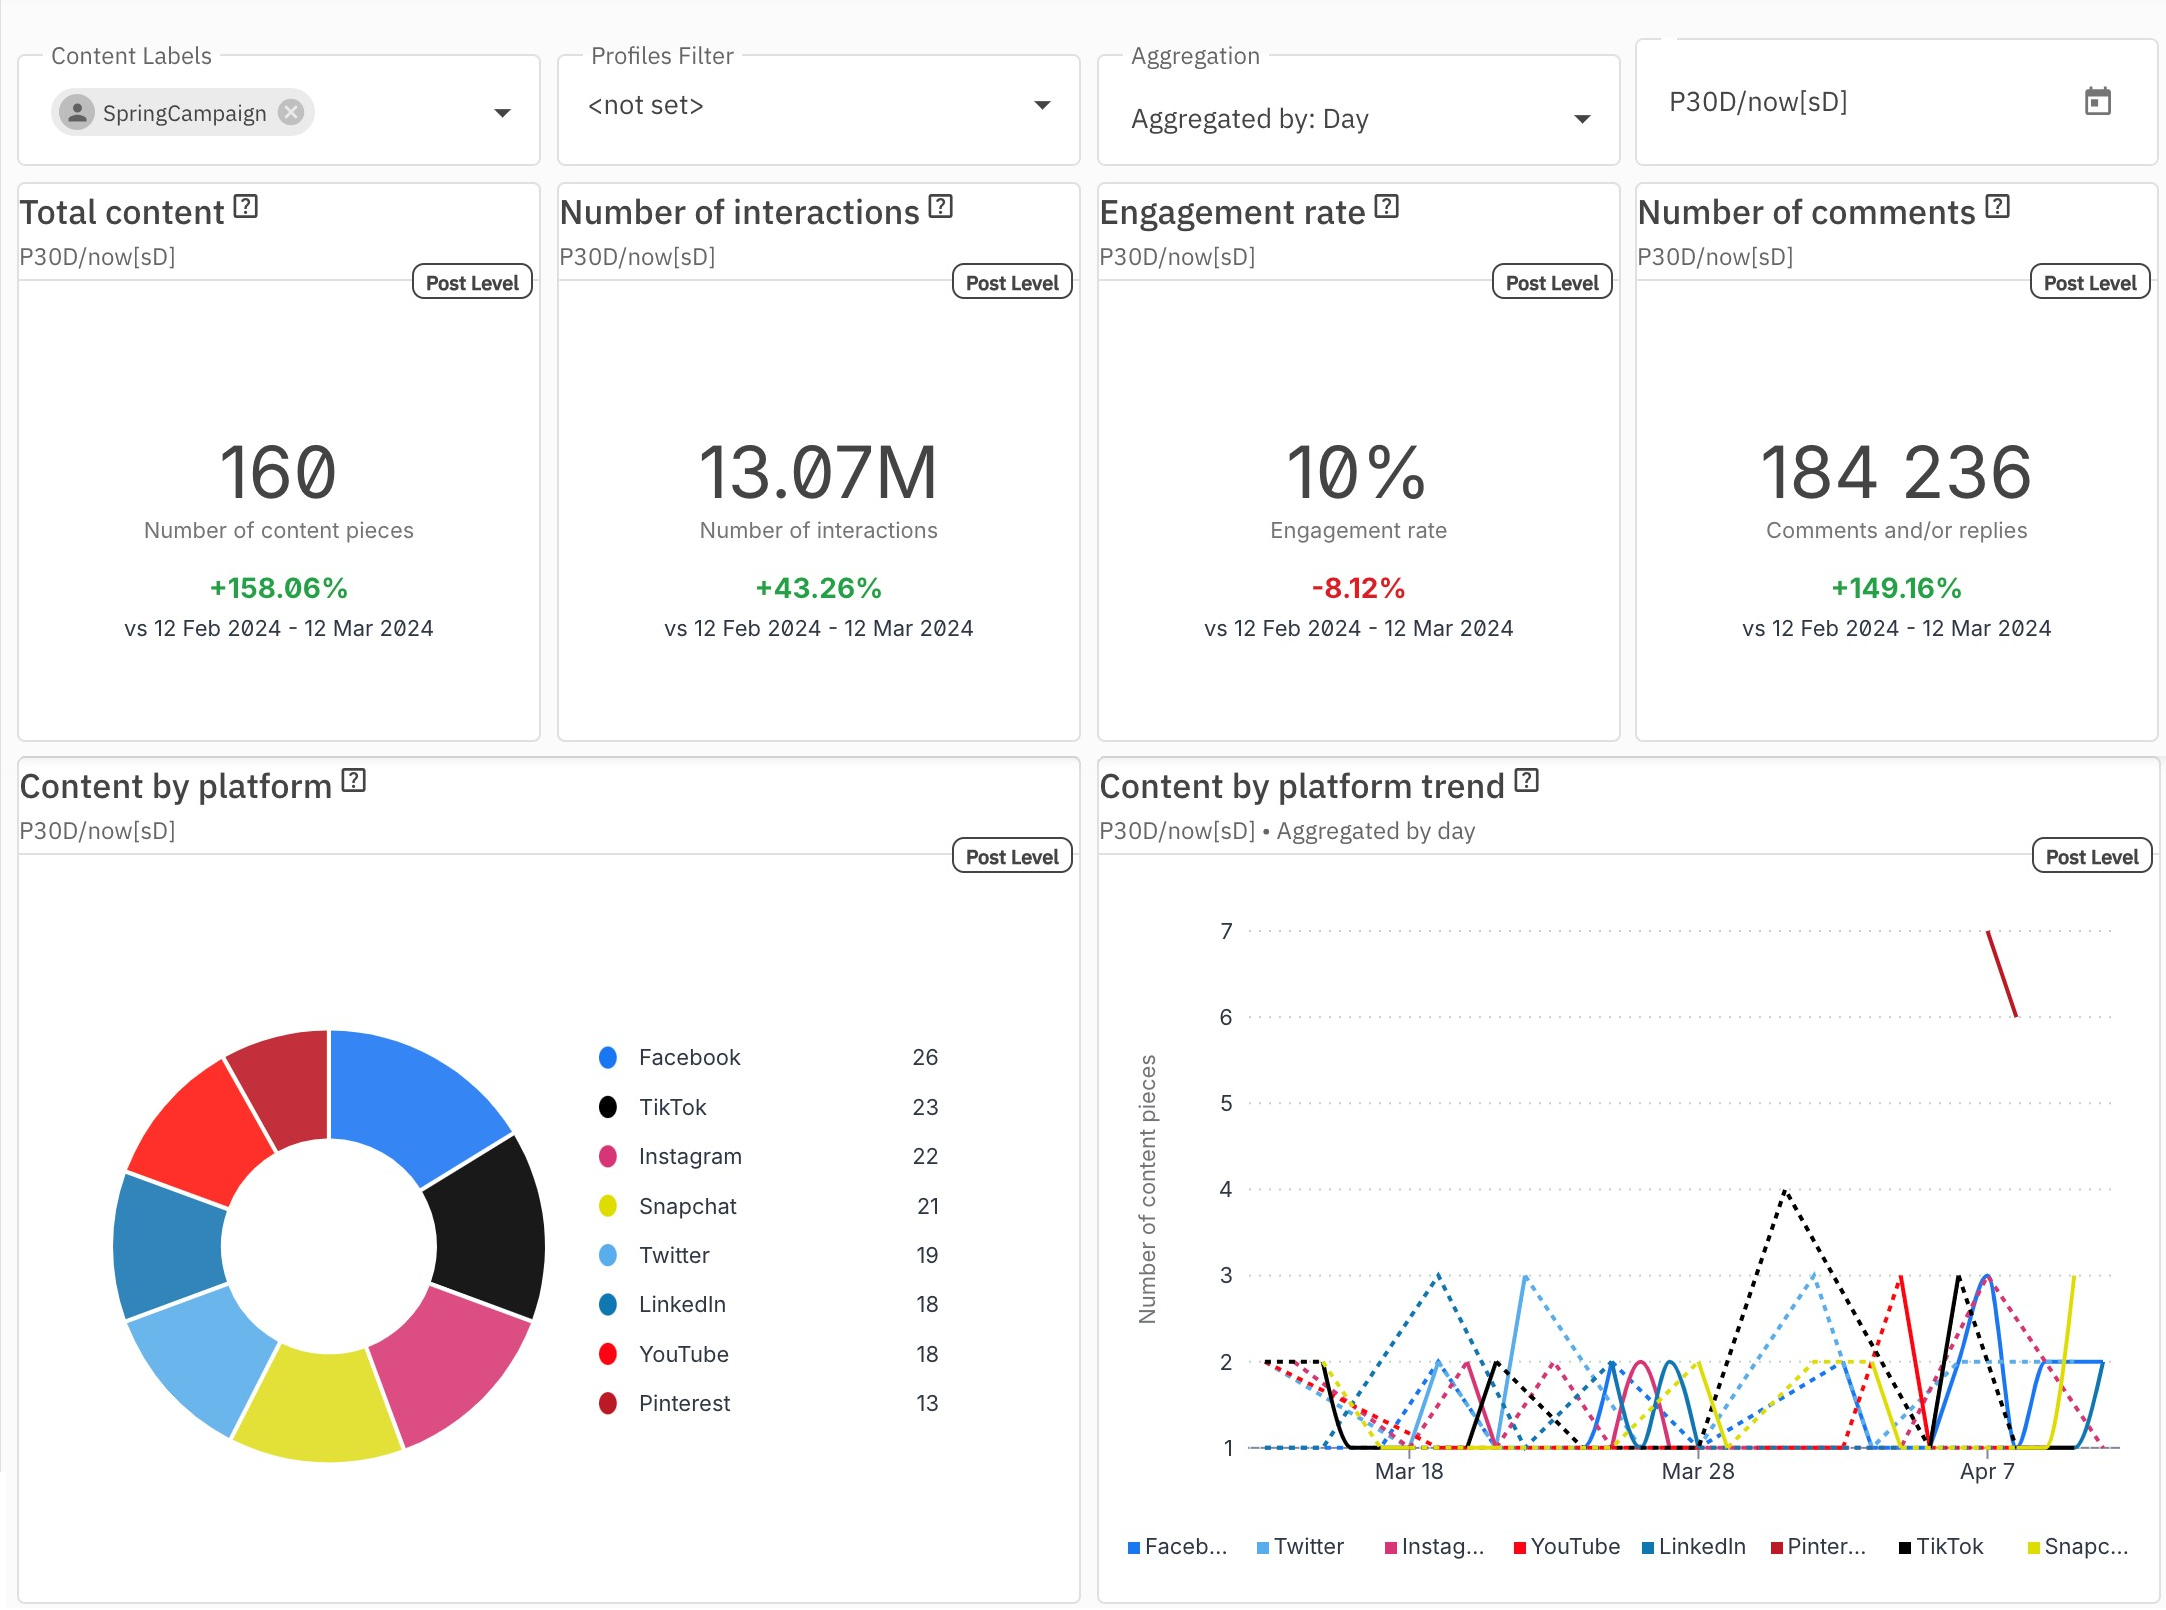
\includegraphics[width=1\textwidth]{pictures/omni-studio.png}
	\caption{Dashboard v Omni Studiu}
	\label{fig:omniStudioDashboard}
\end{figure}
Vidíme, že dasboard obsahuje nejen vizualizace, ale i ovládací prvky. Každý tento widget má svoje jedinečné ID, které je dostupné, pokud se rozklikne nastavení widgetu. Zároveň Omni Studio 
umožňuje uživateli zobrazit konfiguraci grafu (neexpandované), datové requesty (neexpandované) a i samotná data. V jedné ze sekcí widgetu jsou i tzv. debuggovací nástroje, ve kterých se nachází pole JSON parametrů,
které je dodefinovat, aby graf mohl být vykreslen. Na obrázku \ref{fig:omniStudioDashboard} je zřejmé, že uživatel pro realizaci vykreslení musel vybrat hodnoty v ovládacích prvkách (konkrétně 
časovou škálu, časovou agregaci a hodnotu labelu - hodnota pro filtry zůstala nevyplněná, jelikož je nepovinná - udává pouze omezení na datový request, pokud by chtěl uživatel data ještě nějak
dál extrahovat - např. filtrování na základě sociální sítě, typu interakcí apod.). 

Tyto hodnoty se následně převedou do pole JSON objektů a následně se při vizualizaci uplatní. Tím grafy zůstávají dynamické, protože při každé uživatelské interakci se ihned překreslí s novými
daty.

Tyto parametry budou klíčové pro správnou funkcionalitu knihovny - zajistí správné vykreslení a pokud nebudou v rámci aplikace specifikovány nějakými prvky (např. že by uživatelova aplikace obsahovala
inputy/výběrové seznamy pro všechny nespecifikované hodnoty), bude nutné je specifikovat ručně. To bude provedeno předáním přes properties React komponenty.

\subsection{Funkcionalita knihovny}
Knihovna tedy bude obsahovat obecnou komponentu \texttt{<Widget/>}, která bude reprezentovat právě jednu vizualizaci. Bude nutné komponentě předat číslo boardu, číslo widgetu a případně parametry, které 
budou expandovány knihovnou PreJSON v konfiguraci widgetu. Tato komponenta se postará o veškeré fetchování dat a následnou vizualizaci. Jelikož Vision knihovna vizualizuje pouze samotný graf, bude nutné, aby
Widget komopnenta uměla zobrazit i nadpisy, podnadpisy a další prvky obsažené v hlavičce. Bude tedy třeba zajistit základní stylování (např. fonty a velikost písma), ale uživateli bude umožněno vložení CSS stylů
opět přes propsu komponenty - to nabídne uživateli větší možnosti, jak si embedovaný graf sám vystylovat. Postup při vizualizaci bude vypadat přibližně takto:

\begin{enumerate}
	\item Uživatel zadá ID boardu a widgetu + další potřebné parametry
	\item Komponenta provede veškerá potřebná volání - stáhne konfigurace, proběhne expandace konfigů apod.
	\item Aplikují se předané CSS styly 
	\item Výsledné zobrazení grafu
\end{enumerate}

Výsledná knihovna bude přístupná přes npm (Node Package Manager), což zajistí její snadné stažení a použití. Instalace bude vyžadovat pouze nainstalovaného správce balíčků npm a použití budete
detailně vysvětleno v uživatelské dokumentaci.

\section{Návrh UI}

Při navrhování uživatelského rozhraní je třeba myslet na UX (User Experience). Výsledné rozhraní musí být přehledné, uživatelsky přívětivé a nezasekávat se. Pro lepší UX bude rozhraní 
obsahovat nejen sekci pro správu tokenů, ale také sekci pro náhled embedovaných grafů a následné generování zdrojového kódu pro tyto náhledy. Tím se zvýší použitelnost tohoto UI, jelikož 
věci potřebné k embedování sloučí do jednoho UI (tj. bude se jednat o jednostránkovou aplikaci). Ze strany zadavatele je důraz především na funkcionalitu a UX, nikoliv na estetiku. Proto toto bude zohledněno při navrhování.

\subsection{Vytváření tokenů}

K vytvoření tokenů bude sloužit patička stránky. V ní se budou nacházet dvě tlačítka - jedno pro vytvoření Public API tokenu, druhé pro Omni API token. K vytvoření těchto tokenů je třeba být přihlášen v
účtu Suite, jak bylo dřívě zmíněno. Po stisknutí tlačítka bude uživatel přesměrován na stránku, kde udělí patřičné oprávnění, že se pro jeho účet vytvoří token. Po potvrzení se uživateli token uloží
do local storage webového prohlížeče. To umožní okamžitou možnost embedování v UI a zároveň snadnou přístupnost k tomuto tokenu. Pokud bude chtít uživatel token používat ve své aplikaci, jednoduše jej z local storage
zkopíruje k sobě do aplikace, kde jej bude dále moci normálně využívat. To by platilo pro případ, kdy by jeden z tokenů vypršel. Ovšem bude-li uživatel nový a bude nutno vygenerovat oba dva tokeny pro potřebné vizualizace,
bude přidáno tlačítko, které uživateli zkopíruje oba dva tokeny ve formátu .env souboru. Uživatel tedy nebude muset sám hodnoty přepisovat, ale pouze je vloží zkopírované do envu. Zkopírované tokeny
budou ve formátu:
\lstset{style=plainsrc}
\begin{lstlisting}
ACCESS_TOKEN=pis4185dfgfdesfDs5asd
OMNI_API_TOKEN=s5Z9sB=Fd--lK67a44ed12
\end{lstlisting}

\subsection{Náhled vizualizací}
Součástí uživatelského rozhraní bude také sekce pro náhled na vizualizované grafy. Ten bude obsahovat základní uživatelské vstupy (všechny, které bude přijímat výsledná komponenta z naimplementované knihovny), 
díky kterým se vizualizace budou moci rychle ovládat a vykreslovat. Pro rychlé embedování bude vytvořeno i tlačítko, které otevře uživateli dialog, v němž bude vygenerovaný zdrojový kód, kterým by se
v jeho aplikaci daný graf vykreslil. Výstup bude vypadat zhruba takto:

\lstset{style=plainsrc}
\begin{lstlisting}
<Widget widgetID={1598} boardID={12} 
params={{time:"now"}} width={500}/>
\end{lstlisting}


\section{Dokumentace}

Výstupem bude i podrobná dokumentace - a to jak uživatelská, která bude specifikovat použití pro koncové uživatele, tak i programátorská, která bude obsahovat souhrn informací potřebné
pro další vývoj. Dokumentace bude obsahovat následující body:

\begin{enumerate}
	\item Instalaci knihovny a její následnou integraci do uživatelovi aplikace
	\item Stručný návod k používání uživatelského rozhraní pro obnovu tokenů
	\item Sekci pro vývojáře
\end{enumerate}

Přístupu k dokumentaci je několik - od stručného souboru .pdf až po samostatnou webovou aplikaci. Aby dokumentace byla přehledná a snadno rozšiřitelná, bude dokumentace statická stránka
přístupná na veřejné URL adrese. Pro tuto možnost využijeme Docosaurus - generátor statických stránek určen pro generaci právě uživatelských dokumentací. 

Docosaurus umožní ze souborů s příponou .md (soubory běžně používané pro dokumentace v gitových repozitářích) zbuildit statickou webovou stránku, která uživateli poskytne přehledné 
rozhraní. Výsledná dokumentace bude vydána na veřejné internetové stránce, aby k ní byl snadný přístup odkudkoliv.


\chapter{Implementace}
Tato kapitola popisuje implementaci knihovny a uživatelského rozhraní. 
\section{Implementace knihovny}

\subsection{}

\section{Implementace uživatelského rozhraní}


% _____________________________________________________________________________
%
%
%        CHAPTER Závěr
%
% _____________________________________________________________________________
%
\chapter{Závěr}
Aktuálně je praktická část bakalářské práce ve formě, kdy React aplikace dokáže vizualizovat grafy. Grafy lze vizualizovat pomocí playgroundu, kterému bude v budoucnu ještě upraven
frontend. Zároveň aplikace dokáže obnovovat OAuth2 tokeny (jak token pro Emplifi Public Api, který vrací schémata widgetů, tak i token pro Omni API, který vrací data do widgetů). Toto je
udělané pouze formou dvou tlačítek. Ty jsou automaticky vypnuté, pokud jsou tokeny validní - momentálně se uchovávají v local storage webového prohlížeče. Externí zadavatel určí co dále. 
Jsou i vypisovány základní stavy tokenu (platný, neplatný, neexistující) a vizualizace v playground nelze embedovat, dokud tyto tokeny nejsou platné. Playground umožňuje uživatelům widgety
i upravovat - například zadáním CSS stylu či zadáním šířky/výšky. Pro debuggování a kontrolu jsou umožněny i výpisy schémat daného widgetu - ty se ovládají jednoduchým přepínačem. Jsou 
ošetřeny základní chyby, které mohou nastat při vizualizaci (chybějící tokeny, nezadané parametry pro PreJSON apod.). 

Nyní bych rád pokračoval v zefektivnění kódu, dopsáním dokumentačních komentářů, napsáním jednotkových testů pro kritické sekce programu, zlepšení frontendu pro playground a pro rozhraní pro
obnovu OAuth 2.0 tokenů. Zároveň bude třeba ošetřit všechny výjimky, které mohou nastat. Dalším krokem bude převést React aplikaci na knihovnu a domluvit se se zadavatelem, jak pokračovat dále -
například zda-li stačí vizualizovat jednotlivé widgety, nebo celé dashboardy. Jako poslední budou provedeny i funkcionální testy podle scénářů, které budou přiloženy ve finálním odevzdání bakalářské práce.

\appendix
\backmatter
\printbibliography
\listoffigures
\listoftables
\listoflistings
% _____________________________________________________________________________
%
%		BACK COVER
% _____________________________________________________________________________
%
\setbackpageqrcode
\backpage
\end{document}